\documentclass[conference]{IEEEtran}
\IEEEoverridecommandlockouts
\usepackage{cite}
\usepackage{balance}
\usepackage{amsmath,amssymb,amsfonts}
\usepackage{graphicx}
\usepackage{textcomp}
\usepackage{xcolor}
\usepackage{booktabs}
\usepackage{algorithm}
\usepackage{algorithmic}
\usepackage{tikz}
\usetikzlibrary{positioning,arrows.meta,fit,calc}
\usepackage[hidelinks]{hyperref}
\newcommand{\NInst}{30}
\newcommand{\NFeasInst}{30}
\newcommand{\NBinding}{12}
\newcommand{\MeanFeasAssign}{45.0}
\newcommand{\Shots}{32}
\newcommand{\UniBits}{0.00033}
\newcommand{\UniOneHot}{0.0169}
\newcommand{\ExactMs}{0.90}
\newcommand{\SAOpt}{10.0}
\newcommand{\SAFeas}{83.3}
\newcommand{\SAMs}{2.3}
\newcommand{\GreedyOpt}{93.3}
\newcommand{\GreedyFeas}{100.0}
\newcommand{\QuboExact}{93.3}
\newcommand{\QXMeanOnePopt}{0.004}
\newcommand{\QXMeanOnePfeas}{0.074}
\newcommand{\QXMeanOneSucc}{12.2}
\newcommand{\QXMeanOneArgmax}{36.7}
\newcommand{\QXMeanOneNfev}{96}
\newcommand{\QXMeanOneMs}{0.29}
\newcommand{\QXMeanTwoPopt}{0.011}
\newcommand{\QXMeanTwoPfeas}{0.249}
\newcommand{\QXMeanTwoSucc}{27.6}
\newcommand{\QXMeanTwoArgmax}{40.0}
\newcommand{\QXMeanTwoNfev}{479}
\newcommand{\QXMeanTwoMs}{4.22}
\newcommand{\QXMeanThreePopt}{0.024}
\newcommand{\QXMeanThreePfeas}{0.439}
\newcommand{\QXMeanThreeSucc}{48.2}
\newcommand{\QXMeanThreeArgmax}{26.7}
\newcommand{\QXMeanThreeNfev}{721}
\newcommand{\QXMeanThreeMs}{4.03}
\newcommand{\QXMeanFourPopt}{0.040}
\newcommand{\QXMeanFourPfeas}{0.547}
\newcommand{\QXMeanFourSucc}{63.7}
\newcommand{\QXMeanFourArgmax}{40.0}
\newcommand{\QXMeanFourNfev}{750}
\newcommand{\QXMeanFourMs}{8.71}
\newcommand{\QXYMeanOnePopt}{0.054}
\newcommand{\QXYMeanOnePfeas}{0.734}
\newcommand{\QXYMeanOneSucc}{67.1}
\newcommand{\QXYMeanOneArgmax}{3.3}
\newcommand{\QXYMeanOneNfev}{272}
\newcommand{\QXYMeanOneMs}{0.83}
\newcommand{\QXYMeanTwoPopt}{0.093}
\newcommand{\QXYMeanTwoPfeas}{0.722}
\newcommand{\QXYMeanTwoSucc}{77.8}
\newcommand{\QXYMeanTwoArgmax}{13.3}
\newcommand{\QXYMeanTwoNfev}{741}
\newcommand{\QXYMeanTwoMs}{2.97}
\newcommand{\QXYMeanThreePopt}{0.143}
\newcommand{\QXYMeanThreePfeas}{0.743}
\newcommand{\QXYMeanThreeSucc}{81.9}
\newcommand{\QXYMeanThreeArgmax}{16.7}
\newcommand{\QXYMeanThreeNfev}{750}
\newcommand{\QXYMeanThreeMs}{3.73}
\newcommand{\QXYMeanFourPopt}{0.215}
\newcommand{\QXYMeanFourPfeas}{0.795}
\newcommand{\QXYMeanFourSucc}{88.4}
\newcommand{\QXYMeanFourArgmax}{40.0}
\newcommand{\QXYMeanFourNfev}{750}
\newcommand{\QXYMeanFourMs}{5.53}
\newcommand{\QXCvarOnePopt}{0.005}
\newcommand{\QXCvarOnePfeas}{0.132}
\newcommand{\QXCvarOneSucc}{14.6}
\newcommand{\QXCvarOneArgmax}{23.3}
\newcommand{\QXCvarOneNfev}{108}
\newcommand{\QXCvarOneMs}{0.37}
\newcommand{\QXCvarTwoPopt}{0.019}
\newcommand{\QXCvarTwoPfeas}{0.294}
\newcommand{\QXCvarTwoSucc}{44.0}
\newcommand{\QXCvarTwoArgmax}{63.3}
\newcommand{\QXCvarTwoNfev}{577}
\newcommand{\QXCvarTwoMs}{54.22}
\newcommand{\QXCvarThreePopt}{0.037}
\newcommand{\QXCvarThreePfeas}{0.356}
\newcommand{\QXCvarThreeSucc}{65.7}
\newcommand{\QXCvarThreeArgmax}{70.0}
\newcommand{\QXCvarThreeNfev}{728}
\newcommand{\QXCvarThreeMs}{793.23}
\newcommand{\QXCvarFourPopt}{0.060}
\newcommand{\QXCvarFourPfeas}{0.376}
\newcommand{\QXCvarFourSucc}{78.4}
\newcommand{\QXCvarFourArgmax}{66.7}
\newcommand{\QXCvarFourNfev}{706}
\newcommand{\QXCvarFourMs}{5.47}
\newcommand{\QXYCvarOnePopt}{0.067}
\newcommand{\QXYCvarOnePfeas}{0.720}
\newcommand{\QXYCvarOneSucc}{82.7}
\newcommand{\QXYCvarOneArgmax}{6.7}
\newcommand{\QXYCvarOneNfev}{241}
\newcommand{\QXYCvarOneMs}{0.83}
\newcommand{\QXYCvarTwoPopt}{0.099}
\newcommand{\QXYCvarTwoPfeas}{0.712}
\newcommand{\QXYCvarTwoSucc}{93.9}
\newcommand{\QXYCvarTwoArgmax}{20.0}
\newcommand{\QXYCvarTwoNfev}{413}
\newcommand{\QXYCvarTwoMs}{1.78}
\newcommand{\QXYCvarThreePopt}{0.127}
\newcommand{\QXYCvarThreePfeas}{0.672}
\newcommand{\QXYCvarThreeSucc}{97.3}
\newcommand{\QXYCvarThreeArgmax}{36.7}
\newcommand{\QXYCvarThreeNfev}{343}
\newcommand{\QXYCvarThreeMs}{1.88}
\newcommand{\QXYCvarFourPopt}{0.149}
\newcommand{\QXYCvarFourPfeas}{0.664}
\newcommand{\QXYCvarFourSucc}{98.1}
\newcommand{\QXYCvarFourArgmax}{50.0}
\newcommand{\QXYCvarFourNfev}{284}
\newcommand{\QXYCvarFourMs}{1.75}
\newcommand{\XYPfeasMin}{0.722}
\newcommand{\XYPfeasMax}{0.795}
\newcommand{\GainXYoverUni}{12.7}
\newcommand{\GainXYoverX}{5.3}
\newcommand{\ZZX}{14.0}
\newcommand{\ZZXY}{2.0}
\newcommand{\OvPairs}{2.0}
\newcommand{\ScaleMaxQ}{18}
\newcommand{\ScaleXYsix}{0.006}
\newcommand{\ScaleUnisix}{0.0017}
\newcommand{\ScaleXYmsSix}{99.4}
\newcommand{\ScaleExactSix}{8.14}
\newcommand{\ScaleQuboMin}{90}
\newcommand{\NNonBinding}{18}
\newcommand{\XYBind}{0.111}
\newcommand{\XYNonBind}{0.284}
\newcommand{\XYMin}{0.002}
\newcommand{\XYCvarMin}{0.074}
\newcommand{\XYMax}{0.796}
\newcommand{\XYCvarMax}{0.439}
\newcommand{\XBind}{0.039}
\newcommand{\XNonBind}{0.041}
\newcommand{\ScaleXYtwo}{0.694}
\newcommand{\ScaleXtwo}{0.124}
\newcommand{\ScaleXsix}{0.0009}
\newcommand{\ScaleInfeasSix}{1}
\newcommand{\ScaleXYfeasSix}{0.271}
\newcommand{\ScaleXfeasSix}{0.051}
\newcommand{\TrajInst}{10}
\newcommand{\TrajRuns}{200}
\newcommand{\TrajIdealXY}{0.172}
\newcommand{\TrajIdealX}{0.046}
\newcommand{\TrajXYOne}{0.105}
\newcommand{\TrajXOne}{0.033}
\newcommand{\TrajGlobXYOne}{0.086}
\newcommand{\TrajXYTwo}{0.058}
\newcommand{\TrajRatioOne}{3.2}
\newcommand{\NtwoLayer}{14.0}
\newcommand{\CnotLayer}{28}
\newcommand{\CnotFour}{112}
\newcommand{\ExOpt}{ABCB}
\newcommand{\ExOptCost}{80.86}
\newcommand{\ExSecond}{ABBB}
\newcommand{\ExSecondCost}{80.88}
\newcommand{\ExGap}{0.02}
\newcommand{\ExXYOpt}{0.319}
\newcommand{\ExXYSecond}{0.303}
\newcommand{\ExXYFeas}{0.982}
\newcommand{\ExXOpt}{0.049}
\newcommand{\ExXFeas}{0.681}
\newcommand{\ExNFeas}{29}
\newcommand{\NoiseXYOnePct}{0.104}
\newcommand{\NoiseXYOnePctDepth}{4}
\newcommand{\NoiseXOnePct}{0.023}
\newcommand{\NoiseXYTwoPct}{0.050}
\newcommand{\NoiseXYTwoPctDepth}{4}
\newcommand{\NoiseCvarTwoPctDepth}{2}
\newcommand{\NSeeds}{5}
\newcommand{\NPaired}{30}
\newcommand{\SeedXYMean}{0.188}
\newcommand{\SeedXYSd}{0.020}
\newcommand{\SeedXYMin}{0.168}
\newcommand{\SeedXYMax}{0.215}
\newcommand{\SeedXMin}{0.035}
\newcommand{\SeedXMax}{0.048}
\newcommand{\GMMeanFour}{0.139}
\newcommand{\GMCvarFour}{0.117}
\newcommand{\GMFeasFour}{0.815}
\newcommand{\StXYvXMaxP}{8.0\times10^{-6}}
\newcommand{\StXYvXMinP}{2.2\times10^{-8}}
\newcommand{\StXYvXWinsMin}{25}
\newcommand{\StXYvXWinsMax}{29}
\newcommand{\StXYvGMMaxP}{0.74}
\newcommand{\StXYvGMMinP}{0.19}
\newcommand{\StXYvGMWinsMin}{15}
\newcommand{\StXYvGMWinsMax}{20}
\newcommand{\PenBestLam}{0.25}
\newcommand{\PenBestPopt}{0.104}
\newcommand{\PenBestFeas}{0.401}
\newcommand{\PenGain}{2.6}
\newcommand{\SATunedOpt}{80.0}
\newcommand{\SATunedFeas}{90.0}
\newcommand{\SATunedMs}{128}
\newcommand{\ZeroPenInfeasAll}{30}
\newcommand{\LooDonorFour}{0.292}
\newcommand{\LooTrainedFour}{0.215}
\newcommand{\LooMedianFour}{0.001}
\newcommand{\LooNDonors}{2}
\newcommand{\BestFiveFour}{0.297}
\newcommand{\BestFiveEvals}{12,552}
\newcommand{\HoN}{30}
\newcommand{\HoFt}{30}
\newcommand{\HoTrainedFour}{0.163}
\newcommand{\HoFixedFour}{0.306}
\newcommand{\HoFtFour}{0.356}
\newcommand{\HoCumFour}{2,496}
\newcommand{\HoWinsFour}{24}
\newcommand{\HoPFour}{1.7\times10^{-4}}
\newcommand{\HoRatioFour}{1.9}
\newcommand{\HoSuccFixed}{99.99}
\newcommand{\HoSuccTrained}{79.7}
\newcommand{\HoCvarFixed}{0.250}
\newcommand{\HoCvarTrained}{0.138}
\newcommand{\HoCvarWins}{29}
\newcommand{\HoXFixed}{0.036}
\newcommand{\HoXTrained}{0.028}
\newcommand{\HoUniform}{0.0189}
\newcommand{\HoFixedOverX}{11.0}
\newcommand{\CityN}{50}
\newcommand{\CityAll}{60}
\newcommand{\CityNCities}{6}
\newcommand{\CityBinding}{16}
\newcommand{\CityUniform}{0.0123}
\newcommand{\CityQuboExact}{84}
\newcommand{\CityMeanCost}{60}
\newcommand{\CityFixed}{0.221}
\newcommand{\CityTrained}{0.243}
\newcommand{\CityP}{0.92}
\newcommand{\CitySuccFixed}{94.7}
\newcommand{\CitySuccTrained}{75.7}
\newcommand{\CitySuccP}{1.4\times10^{-3}}
\newcommand{\CityTrainedLow}{9}
\newcommand{\CityFixedLow}{0}
\newcommand{\CityEvals}{2,502}
\newcommand{\CityCvarFixed}{0.213}
\newcommand{\CityCvarTrained}{0.122}
\newcommand{\CityCvarP}{1.2\times10^{-6}}
\newcommand{\CityXFixed}{0.052}
\newcommand{\CityXTrained}{0.038}
\newcommand{\SzFiveN}{10}
\newcommand{\SzFiveFixed}{0.216}
\newcommand{\SzFiveTrained}{0.138}
\newcommand{\SzFiveFixedMin}{0.176}
\newcommand{\SzFiveTrainedLow}{3}
\newcommand{\SzFiveWins}{6}
\newcommand{\SzFiveP}{0.105}
\newcommand{\SzFiveUnif}{0.0049}
\newcommand{\SzFiveEvals}{2502}
\newcommand{\SzFiveSuccF}{99.9}
\newcommand{\SzFiveSuccT}{63.2}
\newcommand{\SzFiveCvarN}{10}
\newcommand{\SzFiveCvarFixed}{0.190}
\newcommand{\SzFiveCvarTrained}{0.130}
\newcommand{\SzFiveCvarFixedMin}{0.078}
\newcommand{\SzFiveCvarTrainedLow}{0}
\newcommand{\SzFiveCvarWins}{7}
\newcommand{\SzFiveCvarP}{0.037}
\newcommand{\SzFiveCvarUnif}{0.0049}
\newcommand{\SzFiveCvarEvals}{1866}
\newcommand{\SzFiveCvarSuccF}{98.7}
\newcommand{\SzFiveCvarSuccT}{98.0}
\newcommand{\SzSixN}{10}
\newcommand{\SzSixFixed}{0.079}
\newcommand{\SzSixTrained}{0.060}
\newcommand{\SzSixFixedMin}{0.056}
\newcommand{\SzSixTrainedLow}{6}
\newcommand{\SzSixWins}{7}
\newcommand{\SzSixP}{0.557}
\newcommand{\SzSixUnif}{0.0016}
\newcommand{\SzSixEvals}{2486}
\newcommand{\SzSixSuccF}{91.5}
\newcommand{\SzSixSuccT}{39.1}
\newcommand{\SizeCompare}{at 15 qubits the fixed angles were higher on average but not significantly so ($p=0.105$, Wilcoxon); at 18 qubits the fixed angles were higher on average but not significantly so ($p=0.557$, Wilcoxon).}
\newcommand{\SzNoiseN}{10}
\newcommand{\SzNoiseTraj}{200}
\newcommand{\SzNoiseHalfFixed}{0.239}
\newcommand{\SzNoiseHalfTrained}{0.140}
\newcommand{\SzNoiseHalfWins}{8}
\newcommand{\SzNoiseOneFixed}{0.182}
\newcommand{\SzNoiseOneTrained}{0.108}
\newcommand{\SzNoiseOneWins}{8}
\newcommand{\SizeNoise}{Under two-qubit noise the advantage persisted: at $\epsilon=0.01$ the fixed angles kept $P_{\mathrm{opt}}=0.182$ against 0.108 for per-instance angles (better on 8 of 10 instances).}
\newcommand{\SANSweeps}{60}

\newtheorem{lemma}{Lemma}

\begin{document}

\title{Constraint-Preserving QAOA with Transferable\\
Angles for Flood Shelter Assignment}

\author{\IEEEauthorblockN{Anonymous Author(s)}
\IEEEauthorblockA{\textit{Affiliation withheld for double-blind review}}}

\maketitle

\begin{abstract}
Shelter assignment after a flood disruption is a small capacity-constrained assignment problem that is often proposed for quantum optimization, yet mixer studies use equality constraints on random graphs and train new angles for every instance. We study the Quantum Approximate Optimization Algorithm (QAOA) on 12-qubit instances generated by a flood digital twin after a road closure and a shelter surge, using exact statevector simulation. Over \NPaired{} instances and \NSeeds{} optimizer seeds, a constraint-preserving ring-XY mixer placed \SeedXYMean{}~$\pm$~\SeedXYSd{} of its probability on the optimal plan at depth 4, against at most \SeedXMax{} for the transverse-field mixer, and beat it on at least \StXYvXWinsMin{} of \NPaired{} instances at every depth (Holm-adjusted $p\le\StXYvXMaxP$); tuning the penalty weight did not close the gap, and a Grover mixer was statistically indistinguishable from XY but needs far deeper circuits. Because our cost shift and scaling put every instance on the same energy scale, angles fixed on \NPaired{} development instances and applied unchanged to \HoN{} new instances reached $P_{\mathrm{opt}}=\HoFixedFour$ with no per-instance circuit evaluations, against \HoTrainedFour{} for per-instance training with \HoCumFour{} evaluations. On \CityN{} instances built on the OpenStreetMap road networks of \CityNCities{} flood-prone Indian cities, the same angles matched per-instance training ($\CityFixed$ against $\CityTrained$, not significant) and raised success within 32 shots from \CitySuccTrained\% to \CitySuccFixed\%; at 15 and 18 qubits they avoided the collapses of per-instance training. Exhaustive search solves these instances in \ExactMs~ms, so the results inform the design of hardware studies and imply no quantum advantage.
\end{abstract}

\begin{IEEEkeywords}
QAOA, constraint-preserving mixer, parameter transfer, QUBO, evacuation planning
\end{IEEEkeywords}

\section{Introduction}
When a flood closes roads and fills shelters, an emergency officer must decide again which shelter each evacuation group should go to. The decision couples travel time, flood exposure along the route and the seats left at each shelter. As a binary program it is a capacity-constrained assignment problem, the kind that is routinely encoded as a quadratic unconstrained binary optimization (QUBO) problem \cite{Lucas2014,Glover2019} and offered as an application for near-term quantum optimization \cite{Cadelina2024,Abbas2024}.

Three questions are usually left open in such proposals. First, does the circuit respect the constraints or only penalise their violation? The original QAOA \cite{Farhi2014} explores all $2^n$ bitstrings, most of which are not plans, whereas the quantum alternating operator ansatz \cite{Hadfield2019} keeps the state inside a feasible subspace \cite{WangZ2020,Fuchs2022,Bartschi2020}. Mixer comparisons, however, use equality constraints, while shelter capacity is an inequality that couples groups. Second, must the angles be trained again for every disruption? In an evacuation the instance changes with every closure, and per-instance training costs thousands of circuit evaluations. Third, how does the result compare with ordinary classical methods on instances of realistic shape?

We answer these questions on instances generated by the digital twin of a flood decision-support prototype. Our contributions are:
\begin{enumerate}
\item A shelter-assignment QUBO built from twin state, with a pairwise capacity encoding, a penalty bound, and a cost shift and scaling that place all instances on one energy scale; we measure how often the encoding is exact.
\item A controlled comparison of the transverse-field, ring-XY and Grover mixers under mean-energy and conditional value-at-risk (CVaR) training at depths 1--4, replicated over \NSeeds{} optimizer seeds with paired significance tests and a penalty-weight sweep.
\item An angle-transfer protocol: one angle set per depth, chosen on development instances, is applied unchanged to new disruption instances and to instances on real city road networks and on larger instances, and matches or outperforms per-instance training at no per-instance cost.
\item A gate-level noise study and a comparison with exhaustive search, a greedy rule and tuned simulated annealing, with a scaling run to \ScaleMaxQ{} qubits.
\end{enumerate}
All results come from classical simulation; we make no claim of quantum speed-up.

\section{Related Work}
\textit{Formulations.} Lucas gave Ising forms for many NP-hard problems \cite{Lucas2014}, and Glover \textit{et al.} describe how assignment and capacity constraints become quadratic penalties \cite{Glover2019}. Shelter location and allocation for flood evacuation has long been studied with integer programming \cite{Sherali1991}, and quantum annealing has been applied to disaster resource allocation \cite{Cadelina2024}.

\textit{Mixers.} QAOA alternates a cost unitary and a mixing unitary for $p$ layers \cite{Farhi2014}; a recent review covers its variants \cite{Blekos2024}. Hadfield \textit{et al.} generalised the mixer so that it preserves hard constraints \cite{Hadfield2019}. Wang \textit{et al.} analysed ring and complete XY mixers for one-hot constraints \cite{WangZ2020}, Fuchs \textit{et al.} gave general constructions of constraint-preserving mixers \cite{Fuchs2022} and optimal mixers restricted to a subspace \cite{Fuchs2024}, and Grover mixers move the complexity from the mixer into the preparation of the feasible superposition \cite{Bartschi2020}. Applied studies pair XY mixers with warm starts for vehicle routing \cite{doCarmo2025} and build coverage-preserving mixers for personnel rostering \cite{Gupta2026}.

\textit{Training and transfer.} Angles can be interpolated from depth $p$ to $p{+}1$ \cite{Zhou2020}, CVaR objectives raise the probability of good samples \cite{Barkoutsos2020}, and warm starts use classical solutions \cite{Egger2021}. Optimal angles concentrate across instances of one family \cite{Brandao2018} and transfer between random graphs \cite{Galda2021}; for weighted MaxCut, rescaling the weights lets one parameter set serve many instances \cite{Shaydulin2023}. On hardware, QAOA performance falls with size and depth \cite{Harrigan2021}, and practical advantage in optimization has not been shown \cite{Preskill2018,Bharti2022,Abbas2024}.

\textit{Research gap.} Table~\ref{tab:pos} positions this work. The mixer studies above handle equality constraints, the transfer studies use unconstrained MaxCut with the standard mixer, and the disaster-response work solves a penalty QUBO on an annealer. To our knowledge, angle transfer has not been tested for constraint-preserving mixers on inequality-constrained instances, nor on instances that change with a disruption, and no evacuation study compares mixers against an exact optimum, classical baselines and a gate-level noise model together.

\begin{table}[t]
\caption{Position of this work among closely related studies}
\label{tab:pos}
\centering
\footnotesize
\setlength{\tabcolsep}{2.2pt}
\begin{tabular}{llll}
\toprule
Study & Problem (constraints) & Mixers & Transfer\\
\midrule
\cite{WangZ2020} & graph colouring (one-hot) & X, XY & --\\
\cite{Shaydulin2023} & weighted MaxCut (none) & X & yes\\
\cite{doCarmo2025} & routing (one-hot) & XY + warm start & --\\
\cite{Gupta2026} & rostering (coverage) & X, XY variants & --\\
\cite{Cadelina2024} & disaster routing (penalties) & annealer & --\\
This work & shelters (one-hot, capacity) & X, XY, Grover & held-out\\
\bottomrule
\multicolumn{4}{l}{\scriptsize -- = not part of the reported study.}\\
\end{tabular}
\end{table}

\section{Problem Formulation}
\subsection{Instances from the Digital Twin}
The twin models a corridor with three population zones, nine junctions and three shelters joined by 22 roads. Every road carries a travel time, a flood-depth index and a congestion level drawn from a seed. Shelters have capacities of 120, 90 and 70 people with an initial occupancy of 15--45\%, and groups have 8--22 people. Each instance applies the disruption used in the twin's routing benchmark: road R5 closes and Shelter A receives arrivals equal to half its capacity. For group $g$ and shelter $s$ we take the best open path under the twin's flood- and congestion-weighted edge cost and define
\begin{equation}
c_{gs}=T_{gs}+5H_{gs},
\end{equation}
where $T_{gs}$ is travel time in minutes and $H_{gs}$ the mean flood index along the path. The pair $(g,s)$ is \emph{forbidden} if no open path exists, the shelter has failed, or the group alone exceeds the remaining seats $R_s$. With $G$ groups, binary variables $x_{gs}$ give $n=3G$ qubits. A plan is feasible if every group has exactly one shelter, no forbidden pair is used and $\sum_g n_g x_{gs}\le R_s$ for each shelter, where $n_g$ is the group size.

\subsection{QUBO with Pairwise Capacity}
The capacity constraint is an inequality, which normally needs slack qubits \cite{Glover2019}. We use a pairwise encoding instead. Let $\mathcal{O}=\{(g,h,s): n_g+n_h>R_s\}$ be the pairs of groups that cannot share shelter $s$ and $\mathcal{F}$ the forbidden pairs. With shifted costs $c'_{gs}=c_{gs}-\min_{s'}c_{gs'}$,
\begin{multline}
E(\mathbf{x})=\sum_{g,s}c'_{gs}x_{gs}+P\Big[\sum_g\Big(1-\sum_s x_{gs}\Big)^2\\
+\sum_{(g,s)\in\mathcal{F}}x_{gs}+\sum_{(g,h,s)\in\mathcal{O}}x_{gs}x_{hs}\Big].
\label{eq:qubo}
\end{multline}

\begin{lemma}
With $P=1+\sum_g\max_s c'_{gs}$, every bitstring that breaks a one-hot, forbidden-pair or pairwise-capacity term has higher energy than every bitstring that breaks none of them.
\end{lemma}
\noindent\textit{Proof.} Since $c'_{gs}\ge0$, a bitstring with no violated term has energy at most $P-1$, while a violated term adds at least $P$ to a non-negative cost. \hfill$\blacksquare$

\smallskip
On one-hot states the shift subtracts the constant $\sum_g\min_s c_{gs}$, so the optimal plan is unchanged. We then divide the Hamiltonian by $\Delta=P-1$, which maps the energies of all penalty-free plans into $[0,1]$ for every instance. This scaling later allows angles to be shared between instances (Section~\ref{sec:transfer}). The pairwise encoding misses overloads by three or more groups whose pairs all fit, so a penalty-free plan can still be infeasible; every sampled plan is therefore re-checked exactly before use.

\section{QAOA Variants and Training}
For depth $p$ and angles $\boldsymbol\theta=(\boldsymbol\gamma,\boldsymbol\beta)$, QAOA prepares
\begin{equation}
|\psi(\boldsymbol\theta)\rangle=\prod_{k=1}^{p}e^{-i\beta_k B}\,e^{-i\gamma_k \hat E/\Delta}\,|\psi_0\rangle,
\end{equation}
where $\hat E$ is diagonal with entries $E(\mathbf{x})$. Substituting $x_q=(1-Z_q)/2$ turns (\ref{eq:qubo}) into an Ising Hamiltonian with one $R_Z$ rotation per qubit and one two-qubit $ZZ$ rotation per non-zero coupling.

\textit{Transverse-field (X) mixer.} $B=\sum_q X_q$ and $|\psi_0\rangle=|+\rangle^{\otimes n}$; constraints act only through the penalties.

\textit{Ring-XY mixer.} For each group $g$ with qubits $a_g,b_g,c_g$,
\begin{equation}
B_{\mathrm{XY}}=\sum_{g}\ \sum_{(u,v)\in\{(a_g,b_g),(b_g,c_g),(c_g,a_g)\}}\tfrac12\big(X_uX_v+Y_uY_v\big).
\label{eq:xy}
\end{equation}
Each term swaps amplitude between $|01\rangle$ and $|10\rangle$, so a one-hot group stays one-hot \cite{WangZ2020}. The start state $|W_3\rangle^{\otimes G}$, with $|W_3\rangle=(|100\rangle+|010\rangle+|001\rangle)/\sqrt3$, is the uniform superposition of the $3^G$ one-hot plans \cite{Bartschi2019}. The one-hot penalty is then constant and is dropped. The three ring terms are applied in a fixed order, as in a first-order Trotter step.

\textit{Grover mixer.} $B_{\mathrm{GM}}=|\psi_0\rangle\langle\psi_0|$ with the same start state, so $e^{-i\beta B_{\mathrm{GM}}}=I+(e^{-i\beta}-1)|\psi_0\rangle\langle\psi_0|$ \cite{Bartschi2020}. It mixes all one-hot plans in one step, but each layer needs the inverse state preparation, a phase controlled on all $n$ qubits and the preparation again, which is far deeper than the 12 XY rotations of the ring mixer.

\textit{Objectives and training.} We minimise either $\langle\hat E\rangle$ or the CVaR with $\alpha=0.1$ \cite{Barkoutsos2020}. Sorting bitstrings by energy, $E_{(1)}\le E_{(2)}\le\dots$, with probabilities $\pi_{(k)}$ and cumulative mass $\Pi_k=\sum_{j\le k}\pi_{(j)}$,
\begin{equation}
\mathrm{CVaR}_\alpha=\frac1\alpha\sum_k E_{(k)}\,\min\!\big(\pi_{(k)},\ \max(0,\ \alpha-\Pi_{k-1})\big).
\label{eq:cvar}
\end{equation}
Angles are optimised by COBYLA \cite{Powell1994} with at most 250 evaluations per start, depth by depth (Algorithm~\ref{alg:train}).

\begin{algorithm}[t]
\caption{Depth-progressive training and angle transfer}
\label{alg:train}
\begin{algorithmic}[1]
\small
\STATE \textbf{per-instance training} (instance $j$, mixer $B$, seed $r$):
\FOR{$p=1$ \TO $4$}
\STATE starts $\leftarrow$ two draws $\gamma_k\sim U(0,\pi)$, $\beta_k\sim U(0,\pi/2)$
\STATE \textbf{if} $p>1$ \textbf{then} add INTERP$(\boldsymbol\theta_j^{(p-1)})$ \cite{Zhou2020} to starts
\STATE $\boldsymbol\theta_j^{(p)}\leftarrow$ best COBYLA result on $\langle\hat E\rangle$ or (\ref{eq:cvar})
\ENDFOR
\STATE \textbf{transfer:} for each $p$, pick $\boldsymbol\theta^{\star}_p$ by (\ref{eq:transfer}) on development set $\mathcal{D}$
\STATE apply $\boldsymbol\theta^{\star}_p$ unchanged to every new instance; optionally refine with at most \HoFt{} COBYLA evaluations
\end{algorithmic}
\end{algorithm}

\subsection{Angle Transfer}\label{sec:transfer}
Per-instance training must be repeated after every disruption. Since the scaled Hamiltonians of all instances share the energy range $[0,1]$, we test whether trained angles carry over. Let $\Theta_p=\{\boldsymbol\theta_j^{(p)}:j\in\mathcal{D}\}$ be the angles trained on the development instances. We fix
\begin{equation}
\boldsymbol\theta^{\star}_p=\arg\max_{\boldsymbol\theta\in\Theta_p}\ \frac{1}{|\mathcal{D}|}\sum_{j\in\mathcal{D}}P_{\mathrm{opt}}(j;\boldsymbol\theta),
\label{eq:transfer}
\end{equation}
the trained angle set that works best on average across the development instances, and apply it to new instances without any evaluation on them. We choose among whole trained sets instead of averaging angles coordinate by coordinate, because angles trained on different instances sit in different basins of the periodic landscape; their coordinate-wise median gave $P_{\mathrm{opt}}=\LooMedianFour$ in a leave-one-out test.

\section{Experimental Setup}
\textit{Instances.} The development set $\mathcal{D}$ has \NInst{} instances from twin seeds $42+17i$, $i=0,\dots,29$, using the first four groups ($G=4$, $n=12$); all are feasible, with on average \MeanFeasAssign{} feasible plans among the 81 one-hot plans, and in \NBinding{} of them capacity changes the optimal plan. The held-out set has \HoN{} new instances from $i=30,\dots,59$, which were used for nothing but the final transfer test. For a test across networks we built \CityAll{} further instances (\CityN{} feasible, \CityBinding{} capacity-bound) on the OpenStreetMap road graphs of \CityNCities{} flood-prone Indian cities (Delhi, Chennai, Mumbai, Kolkata, Guwahati and Patna), using each city's mapped zones, shelters and road flood-exposure proxy and the same edge weights and travel-time rule as the prototype's live router. The road data are real; demand is not mapped, so group sizes and seats follow the twin's distributions, and the disruption closes the most flood-exposed road on any zone--shelter path and sends half a shelter's capacity to the first shelter.

\textit{Simulation.} The simulator stores the $2^n$ amplitudes in double precision; the cost unitary is one elementwise phase, the X mixer applies $R_X$ qubit by qubit, and each XY term rotates the precomputed amplitude pairs whose target bits are $01$ and $10$. One evaluation at 12 qubits takes under 10~ms on a laptop. All random choices use fixed seeds.

\textit{Metrics.} $P_{\mathrm{opt}}$ is the probability of measuring an optimal plan, $P_{\mathrm{feas}}$ that of a feasible plan, and success@$N$ $=1-(1-P_{\mathrm{opt}})^N$ the chance that one of $N=\Shots$ shots is optimal. We count objective evaluations, each of which is a batch of circuit executions on hardware.

\textit{Replication and statistics.} Per-instance training was repeated with \NSeeds{} optimizer seeds for the X/mean, XY/mean and XY/CVaR variants; seed 0 reproduces the main run. Mixers are compared per instance with the two-sided Wilcoxon signed-rank test, Holm-corrected over the four depths, and with 95\% bootstrap intervals over instances.

\textit{Baselines.} Uniform sampling of the 81 one-hot plans ($P_{\mathrm{opt}}=\UniOneHot$); exhaustive search; a greedy rule that places the largest group first in its cheapest shelter with seats left; and simulated annealing \cite{Kirkpatrick1983} on (\ref{eq:qubo}) with 20 restarts of 200 sweeps. For the X mixer we also swept the penalty $\lambda P$ with $\lambda\in\{0.25,0.5,1,2\}$.

\section{Results}
\subsection{Mixers, Objectives and Penalties}
Table~\ref{tab:mixers} and Fig.~\ref{fig:popt} give the main comparison. The XY mixer reached $P_{\mathrm{opt}}=\QXYMeanFourPopt$ at $p=4$ in the main run and \SeedXYMean{}~$\pm$~\SeedXYSd{} over \NSeeds{} seeds (range \SeedXYMin--\SeedXYMax), against \SeedXMin--\SeedXMax{} for the X mixer. It was better on \StXYvXWinsMin--\StXYvXWinsMax{} of \NPaired{} instances at every depth (Holm-adjusted $p\le\StXYvXMaxP$), and the ranking held for every seed. Its feasibility stayed between \XYPfeasMin{} and \XYPfeasMax{} at every depth, whereas the X mixer began with $P_{\mathrm{feas}}=\QXMeanOnePfeas$ and spent its layers recovering feasibility.

\begin{table}[t]
\caption{Mixers and objectives at depth 4 (\NPaired{} instances, 12 qubits)}
\label{tab:mixers}
\centering
\footnotesize
\setlength{\tabcolsep}{2.2pt}
\begin{tabular}{lcccccc}
\toprule
Variant & $P_{\mathrm{opt}}$ & 95\% CI & seeds & $P_{\mathrm{feas}}$ & s@\Shots\,\% & Evals\\
\midrule
X, mean & 0.040 & 0.031--0.051 & 0.040 $\pm$ 0.005 & 0.547 & 63.7 & 2046\\
XY, mean & 0.215 & 0.153--0.283 & 0.188 $\pm$ 0.020 & 0.795 & 88.4 & 2513\\
XY, CVaR & 0.149 & 0.126--0.178 & 0.139 $\pm$ 0.013 & 0.664 & 98.1 & 1281\\
Grover, mean & 0.139 & 0.121--0.156 & -- & 0.815 & 96.9 & 2033\\
Grover, CVaR & 0.117 & 0.106--0.127 & -- & 0.563 & 96.2 & 918\\
\bottomrule
\multicolumn{7}{l}{\scriptsize CI: 95\% bootstrap over instances, main run. seeds: mean $\pm$ s.d. over \NSeeds{}}\\
\multicolumn{7}{l}{\scriptsize optimizer seeds. s@\Shots: success@\Shots. Evals: cumulative to $p=4$.}\\
\end{tabular}
\end{table}

\begin{figure}[t]
\centering
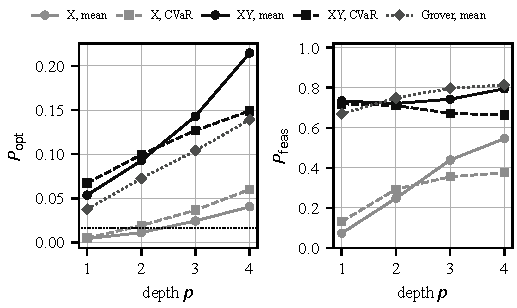
\includegraphics[width=\columnwidth]{fig_popt.pdf}
\caption{Probability of the optimal plan (left) and of any feasible plan (right) against depth, main run. The dotted line is uniform sampling of one-hot plans.}
\label{fig:popt}
\end{figure}

The Grover mixer reached \GMMeanFour{} at $p=4$, and its difference from XY was not significant at any depth (Holm-adjusted $p\ge\StXYvGMMinP$). It spread probability more evenly over instances, so its success@\Shots{} was higher than that of XY with the mean objective, but on hardware it needs a full state preparation and a multi-controlled phase per layer. The ring-XY mixer reaches similar quality with a circuit whose two-qubit gate count per layer equals that of the X variant: \ZZXY{} capacity couplings plus 12 XY rotations, against \ZZX{} $ZZ$ couplings, about \CnotLayer{} CNOTs per layer with all-to-all connectivity.

CVaR training lowered the XY mixer's mean $P_{\mathrm{opt}}$ to \QXYCvarFourPopt{} but raised success@\Shots{} from \QXYMeanFourSucc\% to \QXYCvarFourSucc\%, because it removed the instances with very small $P_{\mathrm{opt}}$: the worst instance rose from \XYMin{} to \XYCvarMin. Those near-zero instances were all capacity-bound, where $P_{\mathrm{opt}}$ averaged \XYBind{} against \XYNonBind{} elsewhere.

A natural objection is that the X mixer was handicapped by its penalty. Lowering the penalty to $\lambda=\PenBestLam$ raised its $P_{\mathrm{opt}}$ by \PenGain$\times$ to \PenBestPopt{} ($\lambda\in\{0.25,0.5,1,2\}$), at a feasibility of only \PenBestFeas, still about half of the XY result; with $\lambda<1$ Lemma~1 no longer guarantees that violations cost more than plans.

\subsection{Angle Transfer to New Disruptions}
In a leave-one-out test on the development set, where (\ref{eq:transfer}) was evaluated without the target instance, the transferred angles gave $P_{\mathrm{opt}}=\LooDonorFour$ at $p=4$ with no evaluation on the target, above per-instance training (\LooTrainedFour) and equal to the best of \NSeeds{} training seeds per instance (\BestFiveFour), which costs \BestFiveEvals{} evaluations per instance. Only \LooNDonors{} distinct angle sets were ever selected.

Table~\ref{tab:transfer} gives the held-out test. Applied unchanged to the \HoN{} new instances, the fixed XY angles reached $P_{\mathrm{opt}}=\HoFixedFour$ at $p=4$, \HoRatioFour$\times$ the \HoTrainedFour{} of per-instance training with \HoCumFour{} evaluations, and were better on \HoWinsFour{} of \HoN{} instances ($p=\HoPFour$). Success within \Shots{} shots rose from \HoSuccTrained\% to \HoSuccFixed\%. Refining the fixed angles with \HoFt{} evaluations raised $P_{\mathrm{opt}}$ to \HoFtFour. CVaR angles transferred as well (\HoCvarFixed{} against \HoCvarTrained, better on \HoCvarWins{} of \HoN). Transfer did not rescue the X mixer (\HoXFixed{} against \HoXTrained), so the gain needs both the constraint-preserving mixer and the shared energy scale.

Per-instance training with a realistic budget therefore stops in poor local optima, as the spread over seeds in Table~\ref{tab:mixers} also shows. For a disruption sequence, training moves offline and each new instance needs only sampling.

\begin{table}[t]
\caption{Held-out transfer: \HoN{} new instances, angles fixed on the development set}
\label{tab:transfer}
\centering
\footnotesize
\setlength{\tabcolsep}{2.2pt}
\begin{tabular}{lccccccc}
\toprule
 & & \multicolumn{2}{c}{trained per instance} & fixed & fixed & \multicolumn{2}{c}{s@\Shots\,\%}\\
Variant & $p$ & $P_{\mathrm{opt}}$ & evals & $P_{\mathrm{opt}}$ & +\HoFt & trained & fixed\\
\midrule
XY, mean & 1 & 0.040 & 278 & 0.089 & 0.110 & 55.5 & 89.6\\
XY, mean & 2 & 0.072 & 996 & 0.162 & 0.226 & 71.8 & 95.4\\
XY, mean & 3 & 0.120 & 1,746 & 0.246 & 0.272 & 76.8 & 99.8\\
XY, mean & 4 & 0.163 & 2,496 & 0.306 & 0.356 & 79.7 & 100.0\\
XY, CVaR & 1 & 0.059 & 310 & 0.063 & 0.115 & 80.7 & 75.7\\
XY, CVaR & 2 & 0.092 & 826 & 0.108 & 0.145 & 93.6 & 88.7\\
XY, CVaR & 3 & 0.126 & 1,246 & 0.180 & 0.178 & 97.9 & 99.6\\
XY, CVaR & 4 & 0.138 & 1,590 & 0.250 & 0.252 & 97.9 & 99.8\\
X, mean & 4 & 0.028 & 2,032 & 0.036 & 0.040 & 50.3 & 63.6\\
\bottomrule
\multicolumn{8}{l}{\scriptsize Fixed angles need 0 evaluations per new instance; +\HoFt{} = refined with \HoFt{} evaluations.}\\
\end{tabular}
\end{table}

\subsection{Transfer to Real Road Networks}
The city instances differ from the twin in network, travel times (mean cost \CityMeanCost{} minutes per pair) and disruption, yet the angles fixed on the twin carried over (Table~\ref{tab:cities}). For the XY mixer with the mean objective, the fixed angles reached $P_{\mathrm{opt}}=\CityFixed$ on the \CityN{} city instances, not significantly different from per-instance training ($\CityTrained$, $p=\CityP$) with \CityEvals{} evaluations, against uniform sampling at \CityUniform. They were more reliable: per-instance training left \CityTrainedLow{} instances with $P_{\mathrm{opt}}<0.01$, the fixed angles \CityFixedLow, so success within \Shots{} shots rose from \CitySuccTrained\% to \CitySuccFixed\% ($p=\CitySuccP$). CVaR angles transferred better than per-instance CVaR training (\CityCvarFixed{} against \CityCvarTrained, $p=\CityCvarP$), and the X mixer stayed far behind (\CityXFixed{} fixed, \CityXTrained{} trained).

\begin{table}[t]
\caption{Fixed angles against per-instance training at $p=4$: held-out twin instances and OpenStreetMap city instances}
\label{tab:cities}
\centering
\footnotesize
\setlength{\tabcolsep}{2.4pt}
\begin{tabular}{lcccccc}
\toprule
 & \multicolumn{2}{c}{twin, \HoN{} new} & \multicolumn{2}{c}{cities, \CityN} & \multicolumn{2}{c}{cities, s@\Shots\,\%}\\
Variant & trained & fixed & trained & fixed & trained & fixed\\
\midrule
XY, mean & 0.163 & 0.306 & 0.243 & 0.221 & 75.7 & 94.7\\
XY, CVaR & 0.138 & 0.250 & 0.122 & 0.213 & 90.6 & 94.9\\
X, mean & 0.028 & 0.036 & 0.038 & 0.052 & 57.1 & 73.0\\
\bottomrule
\multicolumn{7}{l}{\scriptsize Entries are mean $P_{\mathrm{opt}}$ unless marked; fixed angles use 0 evaluations per instance.}\\
\end{tabular}
\end{table}

\subsection{Transfer to Larger Instances and Under Noise}
The angles in (\ref{eq:transfer}) were selected on 12-qubit instances only. We applied them unchanged to \SzFiveN{} new twin instances with five groups (15 qubits) and \SzSixN{} with six groups (18 qubits), and compared them with per-instance training under the same procedure as before (Table~\ref{tab:size}). The fixed angles stayed at least \SzFiveFixedMin{} at 15 qubits and \SzSixFixedMin{} at 18 qubits, far above uniform one-hot sampling, while per-instance training collapsed below $0.01$ on \SzFiveTrainedLow{} and \SzSixTrainedLow{} of the instances. In mean $P_{\mathrm{opt}}$, \SizeCompare{} A sampler fails on exactly these collapsed instances, so success within \Shots{} shots rose from \SzFiveSuccT\% to \SzFiveSuccF\% at 15 qubits and from \SzSixSuccT\% to \SzSixSuccF\% at 18 qubits. \SizeNoise{} With ten instances per size, the test shows that the angles do not break as the problem grows, not that the gain is stable.

\begin{table}[t]
\caption{Angles fixed at 12 qubits, applied at 15 and 18 qubits ($p=4$, new instances)}
\label{tab:size}
\centering
\footnotesize
\setlength{\tabcolsep}{1.9pt}
\begin{tabular}{cccccccccc}
\toprule
 & & & & \multicolumn{2}{c}{trained} & \multicolumn{2}{c}{fixed} & \multicolumn{2}{c}{s@\Shots\,\%}\\
$G$ ($n$) & obj. & inst. & unif. & mean & $<$.01 & mean & min & tr. & fix.\\
\midrule
5 (15) & mean & 10 & 0.0049 & 0.138 & 3 & 0.216 & 0.176 & 63 & 100\\
5 (15) & CVaR & 10 & 0.0049 & 0.130 & 0 & 0.190 & 0.078 & 98 & 99\\
6 (18) & mean & 10 & 0.0016 & 0.060 & 6 & 0.079 & 0.056 & 39 & 92\\
\bottomrule
\multicolumn{10}{l}{\scriptsize $<$.01: instances with $P_{\mathrm{opt}}<0.01$. Fixed angles use 0 evaluations per instance.}\\
\end{tabular}
\end{table}

\subsection{Encoding Exactness}
In every one of the \ZeroPenInfeasAll{} development instances, some infeasible one-hot plan had zero penalty, because three groups whose pairs fit overloaded a shelter together. The minimiser of (\ref{eq:qubo}) was nevertheless the true optimum in \QuboExact\% of instances, because such plans were usually costlier than the optimum. The encoding is therefore approximate, and every sample must be verified exactly.

\subsection{Sensitivity to Gate Noise}\label{sec:noise}
We simulated gate-level noise by quantum trajectories on the first \TrajInst{} instances. In each of \TrajRuns{} runs per circuit every two-qubit gate, including the capacity couplings, the XY rotations and the W-state preparation, fails with probability $\epsilon$ and then applies one of the 15 non-identity two-qubit Pauli operators. Table~\ref{tab:noise} compares this with a global depolarising model, in which the circuit returns its ideal state with probability $F=(1-\epsilon)^{N_2}$ and a uniformly random bitstring otherwise:
\begin{equation}
P_{\mathrm{opt}}^{\epsilon}=F\,P_{\mathrm{opt}}+(1-F)\,n_{\mathrm{opt}}/2^{n}.
\label{eq:noise}
\end{equation}
At $\epsilon=0.01$, of the order reported for current superconducting processors, the XY mixer kept $P_{\mathrm{opt}}=\TrajXYOne$, \TrajRatioOne$\times$ the X mixer's \TrajXOne. The global model is pessimistic (\TrajGlobXYOne) because many Pauli errors, such as late $Z$ errors, barely change the output distribution. Deeper XY circuits stayed ahead of shallower ones at every error rate we tried.

\begin{table}[t]
\caption{$P_{\mathrm{opt}}$ at depth 4 under two-qubit noise (\TrajInst{} instances)}
\label{tab:noise}
\centering
\footnotesize
\setlength{\tabcolsep}{4pt}
\begin{tabular}{lcccc}
\toprule
 & \multicolumn{2}{c}{X mixer} & \multicolumn{2}{c}{XY mixer}\\
$\epsilon$ & traj. & global & traj. & global\\
\midrule
0.001 & 0.045 & 0.044 & 0.162 & 0.161\\
0.005 & 0.038 & 0.036 & 0.128 & 0.121\\
0.01 & 0.033 & 0.028 & 0.105 & 0.086\\
0.02 & 0.023 & 0.016 & 0.058 & 0.043\\
\bottomrule
\multicolumn{5}{l}{\scriptsize traj. = mean over \TrajRuns{} Pauli-error trajectories; global = model (\ref{eq:noise}).}\\
\end{tabular}
\end{table}

\subsection{Classical Baselines and Scaling}
Exhaustive search over the 81 one-hot plans took \ExactMs~ms per instance. The greedy rule found a feasible plan in \GreedyFeas\% of instances and the optimum in \GreedyOpt\%. Simulated annealing with 20 restarts reached the optimum in \SATunedOpt\% and a feasible plan in \SATunedFeas\% in \SATunedMs~ms; a single short run of 60 sweeps reached only \SAOpt\%. Training one QAOA configuration to $p=4$ took several seconds of simulation, so at this size QAOA is not competitive on time and the comparison concerns solution quality per circuit.

Table~\ref{tab:scale} shows the scaling run on the first ten instances with $G=2,\dots,6$ at $p=2$. The XY mixer stayed above uniform one-hot sampling at every size, from \ScaleXYtwo{} at 6 qubits to \ScaleXYsix{} at \ScaleMaxQ, while the X mixer fell below it from 12 qubits on, with a feasibility of only \ScaleXfeasSix{} at \ScaleMaxQ{} qubits. One training run at \ScaleMaxQ{} qubits took \ScaleXYmsSix~s against \ScaleExactSix~ms for exhaustive search; one 18-qubit instance had no feasible plan and was excluded.

\begin{table}[t]
\caption{Scaling with the number of groups ($p=2$, mean objective)}
\label{tab:scale}
\centering
\footnotesize
\setlength{\tabcolsep}{2.4pt}
\begin{tabular}{ccccccccc}
\toprule
$G$ & $n$ & inst. & unif. & X $P_{\mathrm{opt}}$ & XY $P_{\mathrm{opt}}$ & XY $P_{\mathrm{feas}}$ & XY s & exact ms\\
\midrule
2 & 6 & 10 & 0.111 & 0.124 & 0.694 & 0.995 & 2.4 & 0.13\\
3 & 9 & 10 & 0.037 & 0.039 & 0.223 & 0.895 & 2.0 & 0.22\\
4 & 12 & 10 & 0.015 & 0.015 & 0.053 & 0.670 & 2.1 & 0.65\\
5 & 15 & 10 & 0.005 & 0.004 & 0.030 & 0.471 & 5.7 & 2.30\\
6 & 18 & 9 & 0.002 & 0.001 & 0.006 & 0.271 & 99.4 & 8.14\\
\bottomrule
\multicolumn{9}{l}{\scriptsize unif. = uniform one-hot $P_{\mathrm{opt}}$; XY s = simulated training time.}\\
\end{tabular}
\end{table}

\section{Discussion and Limitations}
Three findings bear on moving such problems to hardware. First, the constraint belongs in the mixer: the ring-XY mixer beat the transverse-field mixer on almost every instance and seed, a tuned penalty did not close the gap, and the more expressive Grover mixer gained nothing statistically while needing much deeper circuits. Second, the cost shift and scaling put all instances on one energy scale, which lets a single angle set per depth serve new disruptions better than training each instance from scratch. Third, classical methods solve these instances exactly in milliseconds, and the pairwise capacity encoding admits infeasible penalty-free plans, so a classical verifier must check every sample.

The study has clear limits. The main results are noiseless and the noise model ignores single-qubit and correlated errors, so the probabilities are upper bounds for hardware. The twin is synthetic and the city instances use real roads but sampled demand and one disruption pattern, so transfer to recorded events and to other disruption types remains untested, and shelter accessibility never constrained the plan. The per-instance optimizer had a fixed budget, and evaluations reached the cap at depth 4, so better per-instance angles may exist; transfer matched the best of five seeds, not an exhaustive angle search, and the size test stops at 18 qubits with ten instances per size. The XY mixer was Trotterised in one order, and circuits were not compiled to a hardware gate set or routed.

Threats to validity remain. All variants used the same budget and starts, so the mixer comparison is fair, but the absolute $P_{\mathrm{opt}}$ values depend on that budget. success@$N$ assumes independent shots from an exact distribution. The exhaustive reference makes the optimum known, which a deployment would not have; a deployed verifier can only check feasibility. Future work will test transfer to recorded events and other disruption types, compare slack-variable capacity encodings and run the fixed-angle XY circuit on hardware.

\section{Conclusion}
On shelter-assignment instances drawn from a flood digital twin, a constraint-preserving ring-XY mixer gave QAOA a significantly higher probability of the optimal plan than the transverse-field mixer across instances and optimizer seeds, and matched a Grover mixer with far shallower circuits. Because the cost shift and scaling place every instance on one energy scale, angles fixed on development instances reached $P_{\mathrm{opt}}=\HoFixedFour$ on new disruption instances with no per-instance evaluations, \HoRatioFour$\times$ the result of per-instance training, and matched per-instance training on real road networks of \CityNCities{} cities while finding the optimum within \Shots{} shots far more often. Exhaustive search solves the same instances in about a millisecond, so these results identify formulation and training choices for future hardware experiments, not a present-day advantage.

\section*{Acknowledgment}
The authors thank the OpenStreetMap contributors and Open-Meteo for openly available data used by the digital twin.
In line with the IEEE policy on AI-generated content, the authors disclose that Claude (Anthropic) was used to help edit and restructure the text of all sections and to draft the simulation, experiment and plotting scripts. All experiments use the authors' own software and can be reproduced with fixed seeds. The authors checked every number, claim and reference and take full responsibility for the content.

\balance
\begin{thebibliography}{00}
\bibitem{Lucas2014} A. Lucas, ``Ising formulations of many NP problems,'' \textit{Front. Phys.}, vol. 2, Art. no. 5, 2014, doi: 10.3389/fphy.2014.00005.
\bibitem{Glover2019} F. Glover, G. Kochenberger, and Y. Du, ``Quantum bridge analytics I: A tutorial on formulating and using QUBO models,'' \textit{4OR}, vol. 17, no. 4, pp. 335--371, 2019, doi: 10.1007/s10288-019-00424-y.
\bibitem{Cadelina2024} A. R. Cadeli\~{n}a \textit{et al.}, ``D-Wave implementation of quantum annealing for optimal resource allocation in disaster response operation of Marikina City,'' \textit{ECTI Trans. Comput. Inf. Technol.}, vol. 18, no. 1, pp. 24--33, 2024, doi: 10.37936/ecti-cit.2024181.253577.
\bibitem{Abbas2024} A. Abbas \textit{et al.}, ``Challenges and opportunities in quantum optimization,'' \textit{Nat. Rev. Phys.}, vol. 6, pp. 718--735, 2024, doi: 10.1038/s42254-024-00770-9.
\bibitem{Farhi2014} E. Farhi, J. Goldstone, and S. Gutmann, ``A quantum approximate optimization algorithm,'' arXiv:1411.4028, 2014.
\bibitem{Hadfield2019} S. Hadfield, Z. Wang, B. O'Gorman, E. G. Rieffel, D. Venturelli, and R. Biswas, ``From the quantum approximate optimization algorithm to a quantum alternating operator ansatz,'' \textit{Algorithms}, vol. 12, no. 2, Art. no. 34, 2019, doi: 10.3390/a12020034.
\bibitem{WangZ2020} Z. Wang, N. C. Rubin, J. M. Dominy, and E. G. Rieffel, ``XY mixers: Analytical and numerical results for the quantum alternating operator ansatz,'' \textit{Phys. Rev. A}, vol. 101, no. 1, Art. no. 012320, 2020, doi: 10.1103/PhysRevA.101.012320.
\bibitem{Fuchs2022} F. G. Fuchs, K. O. Lye, H. M. Nilsen, A. J. Stasik, and G. Sartor, ``Constraint preserving mixers for the quantum approximate optimization algorithm,'' \textit{Algorithms}, vol. 15, no. 6, Art. no. 202, 2022, doi: 10.3390/a15060202.
\bibitem{Bartschi2020} A. B\"{a}rtschi and S. Eidenbenz, ``Grover mixers for QAOA: Shifting complexity from mixer design to state preparation,'' in \textit{Proc. IEEE Int. Conf. Quantum Comput. Eng. (QCE)}, 2020, pp. 72--82, doi: 10.1109/QCE49297.2020.00020.
\bibitem{Sherali1991} H. D. Sherali, T. B. Carter, and A. G. Hobeika, ``A location-allocation model and algorithm for evacuation planning under hurricane/flood conditions,'' \textit{Transp. Res. B, Methodol.}, vol. 25, no. 6, pp. 439--452, 1991, doi: 10.1016/0191-2615(91)90037-J.
\bibitem{Blekos2024} K. Blekos \textit{et al.}, ``A review on quantum approximate optimization algorithm and its variants,'' \textit{Phys. Rep.}, vol. 1068, pp. 1--66, 2024, doi: 10.1016/j.physrep.2024.03.002.
\bibitem{Fuchs2024} F. G. Fuchs and R. Pariente Bassa, ``LX-mixers for QAOA: Optimal mixers restricted to subspaces and the stabilizer formalism,'' \textit{Quantum}, vol. 8, Art. no. 1535, 2024, doi: 10.22331/q-2024-11-25-1535.
\bibitem{doCarmo2025} R. S. do Carmo, M. C. S. Santana, F. F. Fanchini, V. H. C. de Albuquerque, and J. P. Papa, ``Warm-starting QAOA with XY mixers: A novel approach for quantum-enhanced vehicle routing optimization,'' arXiv:2504.19934, 2025.
\bibitem{Gupta2026} A. Gupta and S. R. Hassan, ``Constraint-preserving QAOA for personnel rostering: Coverage-preserving and guarded-XY mixer constructions,'' arXiv:2607.09145, 2026.
\bibitem{Zhou2020} L. Zhou, S.-T. Wang, S. Choi, H. Pichler, and M. D. Lukin, ``Quantum approximate optimization algorithm: Performance, mechanism, and implementation on near-term devices,'' \textit{Phys. Rev. X}, vol. 10, no. 2, Art. no. 021067, 2020, doi: 10.1103/PhysRevX.10.021067.
\bibitem{Barkoutsos2020} P. K. Barkoutsos, G. Nannicini, A. Robert, I. Tavernelli, and S. Woerner, ``Improving variational quantum optimization using CVaR,'' \textit{Quantum}, vol. 4, Art. no. 256, 2020, doi: 10.22331/q-2020-04-20-256.
\bibitem{Egger2021} D. J. Egger, J. Mare\v{c}ek, and S. Woerner, ``Warm-starting quantum optimization,'' \textit{Quantum}, vol. 5, Art. no. 479, 2021, doi: 10.22331/q-2021-06-17-479.
\bibitem{Brandao2018} F. G. S. L. Brand\~{a}o, M. Broughton, E. Farhi, S. Gutmann, and H. Neven, ``For fixed control parameters the quantum approximate optimization algorithm's objective function value concentrates for typical instances,'' arXiv:1812.04170, 2018.
\bibitem{Galda2021} A. Galda, X. Liu, D. Lykov, Y. Alexeev, and I. Safro, ``Transferability of optimal QAOA parameters between random graphs,'' in \textit{Proc. IEEE Int. Conf. Quantum Comput. Eng. (QCE)}, 2021, pp. 171--180, doi: 10.1109/QCE52317.2021.00034.
\bibitem{Shaydulin2023} R. Shaydulin, P. C. Lotshaw, J. Larson, J. Ostrowski, and T. S. Humble, ``Parameter transfer for quantum approximate optimization of weighted MaxCut,'' \textit{ACM Trans. Quantum Comput.}, vol. 4, no. 3, Art. no. 19, 2023, doi: 10.1145/3584706.
\bibitem{Harrigan2021} M. P. Harrigan \textit{et al.}, ``Quantum approximate optimization of non-planar graph problems on a planar superconducting processor,'' \textit{Nat. Phys.}, vol. 17, pp. 332--336, 2021, doi: 10.1038/s41567-020-01105-y.
\bibitem{Preskill2018} J. Preskill, ``Quantum computing in the NISQ era and beyond,'' \textit{Quantum}, vol. 2, Art. no. 79, 2018, doi: 10.22331/q-2018-08-06-79.
\bibitem{Bharti2022} K. Bharti \textit{et al.}, ``Noisy intermediate-scale quantum algorithms,'' \textit{Rev. Mod. Phys.}, vol. 94, no. 1, Art. no. 015004, 2022, doi: 10.1103/RevModPhys.94.015004.
\bibitem{Bartschi2019} A. B\"{a}rtschi and S. Eidenbenz, ``Deterministic preparation of Dicke states,'' in \textit{Fundamentals of Computation Theory} (LNCS, vol. 11651). Cham, Switzerland: Springer, 2019, pp. 126--139, doi: 10.1007/978-3-030-25027-0\_9.
\bibitem{Powell1994} M. J. D. Powell, ``A direct search optimization method that models the objective and constraint functions by linear interpolation,'' in \textit{Advances in Optimization and Numerical Analysis}, S. Gomez and J.-P. Hennart, Eds. Dordrecht, The Netherlands: Kluwer, 1994, pp. 51--67, doi: 10.1007/978-94-015-8330-5\_4.
\bibitem{Kirkpatrick1983} S. Kirkpatrick, C. D. Gelatt, and M. P. Vecchi, ``Optimization by simulated annealing,'' \textit{Science}, vol. 220, no. 4598, pp. 671--680, 1983, doi: 10.1126/science.220.4598.671.
\end{thebibliography}

\end{document}
